\documentclass[12pt]{report}
\usepackage[utf8]{inputenc}
\usepackage{titlesec}
\usepackage{hyperref}
\usepackage{apacite}
\usepackage{amsmath}
\usepackage{float}
\usepackage{multirow}
\usepackage{algpseudocode}
\usepackage{algorithm}
\usepackage{booktabs}
\usepackage[a4paper, total={7in, 10in}]{geometry}
\usepackage{graphicx}
\usepackage{titlesec}
\graphicspath{{images/}}
\usepackage{mathptmx}
\usepackage{setspace}
\begin{document}
\singlespacing

\begin{titlepage}
   \begin{center}

        \vspace*{1.5cm}
    
        
\includegraphics[scale=0.3]{mmu-logo.png}
    
       \vspace{1cm}

        \Large
        
       TPT1201 - RESEARCH METHODS IN CS

       \LARGE

       \vspace{1cm}

       \textbf{DDoS Attack Detection Method Based on Improved KNN With the Degree of DDoS Attack in Software-Defined Networks}

       \vspace{1cm}

       Assignment 1

       \vspace{1cm}

       by

       \vspace{1cm}

       \textbf{NUR AYU AMIRA BINTI IDRIS}

       \vspace{1cm}

       \textbf{1201200722}

        \vspace{1cm}

        Trimester 1 - 2022/2023

        \vspace{1cm}

        Bachelor of Computer Science
            
   \end{center}
\end{titlepage}

\section{INTRODUCTION}
Distributed Denial-of-Service, or DDoS, has recently garnered much attention in cyberspace. Software Defined Networking (SDN) principles and techniques have been introduced and extensively studied in recent years. The SDN controller is the most susceptible component to DDoS attacks. Distributed Denial-of-Service (DDoS) aims to block authorized users from network resources. Moreover, the recently developed Software Defined Networking (SDN) offers a new perspective on reevaluating the defence against DDoS attacks. This paper has suggested two methods for detecting DDoS attacks in SDN. One method uses the degree of the DDoS attack as a criterion for determining whether it was a DDoS attack. The other method detects DDoS attacks using an enhanced version of the K-Nearest Neighbors (KNN) algorithm derived from Machine Learning (ML). It provided approaches that can identify DDoS attacks more effectively than other methods based on the results of both the theoretical analysis and the experimental findings on datasets.

\section{PROBLEM STATEMENT AND OBJECTIVES}
Distributed denial of service (DDoS) attacks have been a severe problem to network availability for decades, and there is still no defence mechanism to stop them. The problem studied in this paper is how to detect DDoS attacks in the SDN network effectively. The objectives of the authors’ vital commitments in this paper are to provide a few features and conduct an analysis of the traffic behaviour during a DDoS attack to provide a solution for DDoS detection in an SDN network. In this paper, the authors have proposed four features to evaluate DDoS attack detection while the SDN controller is under attack (flow length, flow duration, flow size, and flow ratio). Next, the authors proposed the degree of attack is a new algorithm for identifying DDoS attacks. This algorithm is called DDADA. Finally, a machine learning–based detection method called DDAML is used to detect DDoS attacks.

\section{RELATED PRIOR RESEARCH WORKS}
Some related works have been on DDoS attack detection methods in the SDN network. For instance, \cite{Shin}  presented a DoS attack on an SDN by separating its control and data plane logic.  Additionally, a network scanning tool was built to identify an SDN network. The scanner could scan the network to change the network header fields. 

Next, \cite{Fonseca} indicated that an attacker sends IP packets with random headers to disrupt the SDN controller in a DDoS attack. This research uses a secondary controller for robustness. DDoS detection was needed since the secondary controller could be attacked. As a result, \cite{Yao}, using several controllers may cause cascading controller faults, making DDoS attacks unsolvable.

\cite{Lin}, suggested using the SDN to detect DDoS attacks. Their approach combined sFlow with three Openflow management tools to find unusual network traffic. As a result, their suggested method's deployment and operation were complicated.\cite{Saied}, suggested an ANN algorithm to recognize Dos attack. Their approach was complicated and ineffective because the packet protocol needed to be distinguished.

\cite{Ye}, recommended combining different Support Vector Machine classification techniques (also known as SVM) to construct the DDoS attack model. The researchers’ approach brought six different feature values—SSIP, SSP, SDFP, SDFB, SFE, and RPF—into play. The findings of their experiments showed that the ICMP traffic had a high false alarm rate, in contrast to the TCP and UDP traffic, which both had low false alarm rates.

Finally, \cite{Cui} suggested a method for detecting the DDoS attack using the CIC-SVM classification algorithm, which stands for Cognitive-Inspired Computing and Support Vector Machine. The researchers’ detection precision still has to be increased.  


\section{RESEARCH METHODOLOGY/ALGORITHMS USED BY THE RESEARCHER}

% 1 Method
\subsection{FEATURES FOR ATTACK TYPES}

The traffic behaviour shows the change in the SDN Network following the attack. Therefore, in this paper, the authors use the flow length, flow duration, flow size, and flow rate as objects to be monitored and investigated in the SDN network, as shown in Table ~\ref{tab:featurestable}.\\

\begin{table}[H]
    \centering
    \begin{tabular}{c c}
    \toprule
    Feature & Meaning \\
    \midrule
    Flow length & number of Packet \\
    Flow duration & the time interval in flow \\
    Flow size & Bytes in flow \\
    Flow rate & Packets per second \\
    \bottomrule
    \end{tabular}
    \caption{Features used in the SDN network and observed in this paper.}
    \label{tab:featurestable}
\end{table}

\subsubsection{INFLUENCE OF TRAFFIC BEHAVIOR AFTER ATTACK}
The entropy method \cite{Rood} was a flexible and fast way to estimate the baseline distribution and detect anomalies. This part uses entropy to identify DDoS attack traffic. Eq.(~\ref{eqn:eqn1}) provides entropy: 

\begin{equation}
    {Entropy(S) = \sum _{i=1}^{n} \nolimits - P_{i} log_{2} P_{i}}
    \label{eqn:eqn1}
\end{equation}

where: \emph{Entropy} \emph{(S)} is a function and Pi is a priori probability. The authors identified the most effective feature in a set of training feature vectors for differentiating between the classes that need to be learned. Eq.(~\ref{eqn:eqn2}) determines this \emph{NGain}: \\

\begin{equation}
    {NGain(S,F) = \frac{Gain(S,F)- max(Gain(S,F))}{max (Gain(S,F)) - min (Gain(S,F))}}
    \label{eqn:eqn2}
\end{equation}

\emph{Theorem 1:} After the DDoS attack, the sample space of flow length entropies for distinct flows is the same.\\

\emph{Proof 1:} The entropy of the flow length $e_{t}(len)$ is given in Eq.(~\ref{eqn:eqn3}).

\begin{equation}
    {e_{t}(len=1) = - \sum _{i=l}^{\Theta} \nolimits e(len = i)c^{l}_{i}p^{l}(1-p)^{i-1}log_{2}P_{i}}
    \label{eqn:eqn3}
\end{equation}

\emph{Theorem 2:} The DDoS attack will affect the flow features' entropy, which the NGain can reflect.\\

\emph{Proof 2:} Suppose that the entropy of the flow feature is $e(ff)$ before the DDoS attack, then after the attack, the entropy of the flow length $e_{t}(ff)$ is given as in Eq.(~\ref{eqn:eqn4}). below:

\begin{equation}
    {e_{t}(ff = m) = - \sum _{i=m}^{\Theta} \nolimits e(ff = m)c^{m}_{i}p^{m}(1-p)^{i-1}log_{2}P_{i}}
    \label{eqn:eqn4}
\end{equation}

DDoS attacks increase SDN network flow length, duration, size, and rate. Then, m in Eq.(~\ref{eqn:eqn4}). increases, and \emph{Gain} increases. The \emph{NGain} value will also be increased. \\

Figure~\ref{fig:ngain} shows the \emph{NGain} values for different features in 8-time intervals, where every three times is considered a time interval. 

\begin{figure}[H]
    \centering
    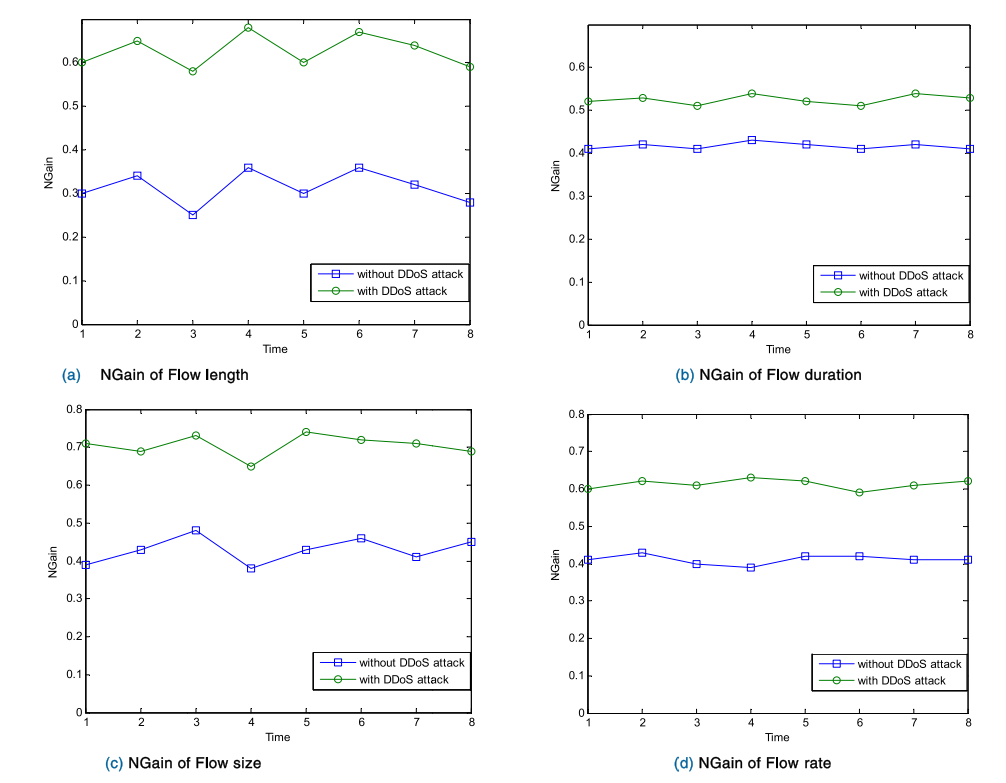
\includegraphics[scale=0.4]{fig6.png}\\
    \caption{NGain values for different features.}
    \label{fig:ngain}
\end{figure}

\subsection{DDOS DETECTION ALGORITHM IN SDN}
%2 method
\subsubsection{DDoS DETECTION ALGORITHM BASED ON DEGREE OF ATTACK}

In this section, the author introduces efficient DDoS detection in an SDN network and describes the related definitions in detail. \\ 

\emph{Definition 1:} The degree of a DDoS attack on an SDN, assuming it has the four features \emph{f1, f2, f3,} and \emph{f4}. Eq.(~\ref{eqn:eqn5}). is used to characterize the DDoS attack's degree \emph{(D)} in the SDN: where: n equals 4 in this paper.\\

\begin{equation}
    {D = \frac{1}{n}\sum _{i=1}^{n} \nolimits N(fi)}
    \label{eqn:eqn5}
\end{equation}

\emph{Definition 2} : Let's say a flow is specified as \emph{F}, and \emph{$f_{t}$} represents the flow's \emph{NGain} at time \emph{t}. The calculation formula to identify the DDoS attacks in the SDN.This measurement is provided as follows: \\

\begin{figure}[H]
    \centering
    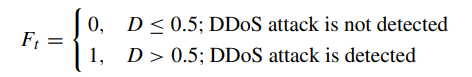
\includegraphics[scale=0.4]{fig8.png}
\end{figure}

The authors conclude that the flow is an attack flow at time t if $D > 0.5$, and the DDoS attack hit the SDN network. Otherwise, the authors determine that the flow is not an attack flow at time t if $D\leq 0.5$. Figure~\ref{fig:gener} shows DDoS attack generation and detection. \\

\begin{figure}[H]
    \centering
    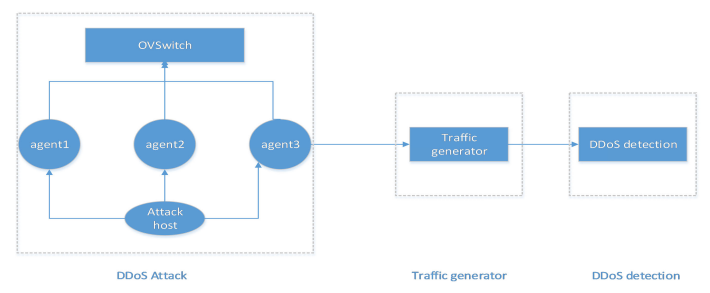
\includegraphics[scale=0.5]{fig9.png}\\
    \caption{DDoS attack generation and detection.}
    \label{fig:gener}
\end{figure}

Finally, Algorithm~\ref{alg:algo1} shows the pseudo-code of the DDoS Detection Algorithm based on the Degree of Attack (DDADA).

\begin{center}
\begin{minipage}{0.5\textwidth}
  \begin{algorithm}[H]
\caption{DDADA Algorithm}
\label{alg:algo1}
\begin{algorithmic}[1]
    \State \textbf{Begin}
    \If {t $\epsilon$ T} 
    \State Calculate D using Eq.(5);
    \If {D $>$ 0.5}
    \State \textbf{network is attacked by DDoS;}
    \Else
    \State \textbf{network is normal;}
    \EndIf
    \EndIf
    \State \textbf{End}
\end{algorithmic}
\end{algorithm}  
\end{minipage}
\end{center}

%3 method
\subsubsection{DDoS DETECTION ALGORITHM BASED ON MACHINE LEARNING}

In this section, the authors propose another algorithm to detect DDoS in the SDN environment to improve the research further. The methods for detecting attacks based on Machine Learning (ML) have been widely used in traditional networks. This section proposes an improved K-Nearest Neighbors identification algorithm (KNN). Eq.(~\ref{eqn:eqn6}). defines the flow distance $x_{i}$ and $x_{j}$ (i.e., $d(x_{i}, x_{j})$) with the following mathematical formula:

\begin{equation}
    {d(x_{i},x{j})=\sqrt{\sum _{m=1}^{n} \nolimits (a_{m}(x_{i})-a_{m}(x_{j})})^{2}}
    \label{eqn:eqn6}
\end{equation}

Let $f(x_{p})$ be the final identification result in Eq.(~\ref{eqn:eqn7}).

\begin{equation}
    {f(x_{p})\leftarrow arg_{v\epsilon V}max\sum _{i=1}^{k} \nolimits D(v,f(x_{i}))}
    \label{eqn:eqn7}
\end{equation}

Figure~\ref{fig:casesknn} (case 2) shows that $f (x_{p})$ will not get the outcome when $f (x_{1})$ = 0, $f (x_{2})$ = 1, $f (x_{3})$ = 0, and $f (x_{4})$ = 1. The authors' use Eq.(~\ref{eqn:eqn8}) weight $w$ to fix this: 

\begin{equation}
    {w=\frac{1}{d(x_{p},x_{i})}}
    \label{eqn:eqn8}
\end{equation}

\begin{figure}[H]
    \centering
    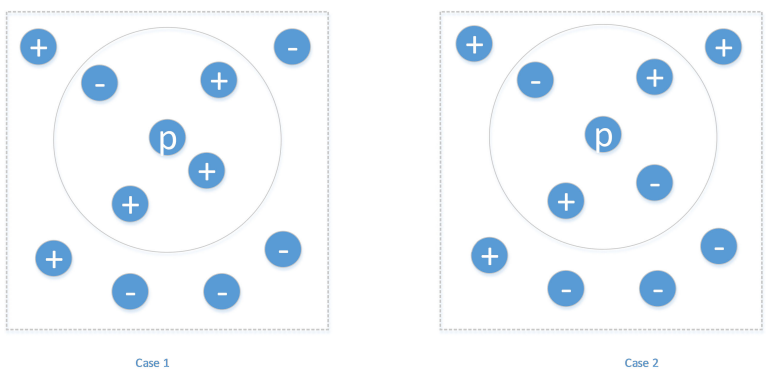
\includegraphics[scale=0.4]{fig13.png}\\
    \caption{Two cases for KNN.}
    \label{fig:casesknn}
\end{figure}


Then, Eq.(~\ref{eqn:eqn9}) can be further expressed as follows: \\

\begin{equation}
    {f(x_{p})\leftarrow arg_{v\epsilon V} max \sum_{i=1}^{k} \nolimits wD(v,f(x_{i}))}
    \label{eqn:eqn9}
\end{equation}


Eq.(9) shows that weight $w$ can solve the Figure~\ref{fig:casesknn} problem (case 2). If $x_{p}$ and $x_{i}$ are the same, then $d(x_{p}, x_{i})$ = 0, $ \lim _{d} \to _{0}$, $w \to \infty $ and $w$ cannot be better computed. The authors define $x_{p}$ = $x_{i}$ when $d(x_{p}, x_{i})$ = 0. The mathematical formula for $f (x_{p})$ is below here. \\ 

\begin{figure}[H]
    \centering
    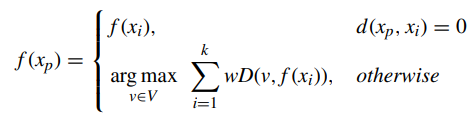
\includegraphics[scale=0.5]{fig16.png}
\end{figure}

Eq.(~\ref{eqn:eqn10})  redefining $w$ as $t = d(x_{p}, x_{i})$ improves weight $w$. Thus, the issue cannot be improved. \\

\begin{equation}
    {w = \frac{1}{e^{t}} = \frac{1}{e^{d(x_{p},x_{i})}}}
    \label{eqn:eqn10}
\end{equation}


To evaluate the authors’ enhanced weight-efficient method, the researchers have defined the weight $w$ in Eq.(9) as $w1$ and the weight $w$ in Eq.(12) as $w2$. Figure~\ref{fig:gauss} shows that the Gauss distribution weight parameter $w2$ better represents the function than $w1$.\\

\begin{figure}[H]
    \centering
    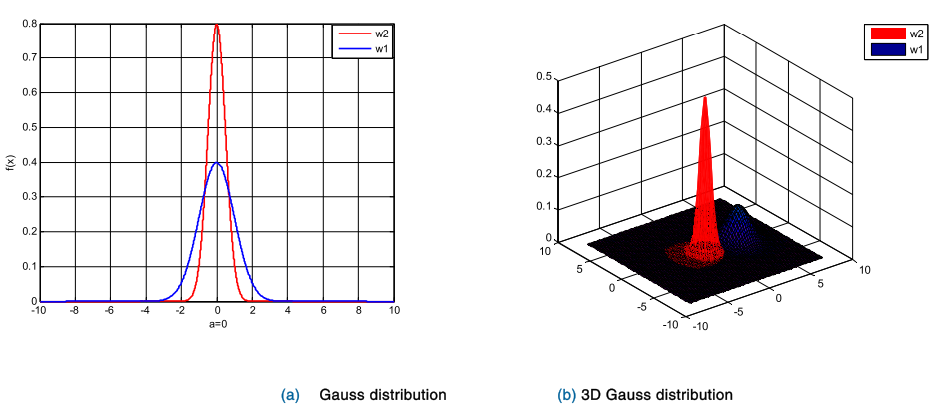
\includegraphics[scale=0.4]{fig18.png}\\
    \caption{Two Gauss distributions for KNN.}
    \label{fig:gauss}
\end{figure}

The authors’ proposed Algorithm~\ref{alg:algo2}, shown in DDoS Detection  based on Machine Learning, solves this detection challenge (DDAML).

\begin{center}
\begin{minipage}{0.5\textwidth}
  \begin{algorithm}[H]
\caption{DDAML Algorithm}
\label{alg:algo2}
\hspace{\algorithmicindent} \textbf{Input:}\textbf{Training\_samples}\\
\hspace*{\algorithmicindent} \textbf{Output:}\textbf{Class label}
\begin{algorithmic}[1]
    \State \textbf{Begin}
    \If {flow $x_{p}$ in training\_samples $f$} 
    \State { \textbf{for} $i=0, i++, i<n$}
    \State {compute $d(x_{p},x{i}$ ;}
    \If {$x_{p}==x_{i}$ }
    \State{$f(x_{p})=f(x_{i}$}
    \Else
    \State{according to Eq.(5) and (9)}
    \State{$f(x_{p}) = arg max_{v}\epsilon v \sum _{i=1}^{k} \nolimits wD(v,f(x_{i}))$}
    \State \Return {$f(x_{p})$}
    \EndIf
    \State{\textbf{end for}}
    \EndIf
    \State \textbf{End}
\end{algorithmic}
\end{algorithm}  
\end{minipage}
\end{center}

\section{PERFORMANCE EVALUATION AND DISCUSSION ON THE RESULTS AND CONTRIBUTIONS BY THE RESEARCHER}
This section evaluates and tests DDoS detection in the SDN.  The authors simulated the proposed algorithms on a Floodlight, an OpenFlow controller. Figure~\ref{fig:topo} shows the authors' small network topology with one server, ten clients (nine agents, and one DDoS user). \\

\begin{figure}[H]
    \centering
    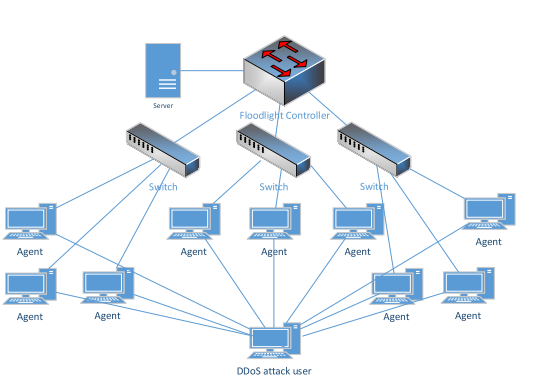
\includegraphics[scale=0.4]{fig20.png}\\
    \caption{Simulation network topology.}
    \label{fig:topo}
\end{figure}

\subsection{EXPERIMENTAL DATA}
The network traffic is 70\% UDP, 20\% TCP, and 10\% ICMP. hping3 produces TCP, UDP, and ICMP flood attack traffic. Table~\ref{tab:exdata} shows the experimental data. 

\begin{table}[H]
    \centering
    \begin{tabular}{l r}
    \toprule
    Type of attack & Data \\
    \midrule
    TCP flood & 1000 \\
    UDP flood & 300  \\
    ICMP flood & 100 \\
    \bottomrule
    \end{tabular}
    \caption{Experimental Data.}
    \label{tab:exdata}
\end{table}


\subsection{MEASUREMENTS EVALUATION}
In this subsection, the authors present DDoS attack detection performance measurements for evaluation. Following is how these measurements are expressed: \\ 

\begin{equation}
    {TPR=\frac{TP}{TP+FN}}
    \label{eqn:eqn11}
\end{equation}

\begin{equation}
    {FPR=\frac{FP}{FP+TN}}
    \label{eqn:eqn12}
\end{equation}

\begin{equation}
    {Precision = \frac{TP}{TP+FP}}
    \label{eqn:eqn13}
\end{equation}

\begin{equation}
    {Precision = \frac{TP}{TP+FP}}
    \label{eqn:eqn14}
\end{equation}

\begin{equation}
    {Recall = TPR = \frac{TP}{TP+FN}}
    \label{eqn:eqn15}
\end{equation}

\begin{equation}
    {F - measure = \frac{2*Recall*Presion}{Recall+Precison}}
    \label{eqn:eqn15}
\end{equation}

\subsection{PERFORMANCE EVALUATION AND RESULTS}
This study evaluates outcomes based on detection accuracy, Receiver Operating Characteristic (ROC), and Area Under the ROC Curve (AUC). Table 3 compares DDADA and DDAML algorithms to the NB \cite{Eibe}, KNN \cite{Daniel}, SVM \cite{Ye}, and CIC SVM \cite{Cui}. 

Table~\ref{tab:eva} shows that DDADA and DDAML algorithms have TPR values of 0.987 and 0.994, respectively, greater than the other techniques. As shown in Table~\ref{tab:eva}, the DDADA and DDAML algorithms have lower FPR values than the other evaluated methods (0.016 and 0.009, respectively), indicating lesser error classifications. The algorithms also have higher Precision, Recall, and F-measures. Table 3 shows the algorithms' TPRs.


\begin{table}[H]
\centering
\begin{tabular}{cccccc}
\hline
\multirow{2}{*}{Method} & \multicolumn{5}{c}{Evaluation}                 \\ \cline{2-6} 
                        & TPR   & FPR   & Precision & Recall & F-measure \\ \hline
NB                      & 0.982 & 0.024 & 0.981     & 0.982  & 0.9815    \\
KNN                     & 0.985 & 0.018 & 0.983     & 0.985  & 0.984     \\
SVM                     & 0.985 & 0.018 & 0.9835    & 0.985  & 0.9842    \\
CIC-SVM                 & 0.986 & 0.017 & 0.9846    & 0.986  & 0.9853    \\
DDADA                   & 0.987 & 0.016 & 0.985     & 0.987  & 0.986     \\
DDAML                   & 0.994 & 0.009 & 0.993     & 0.994  & 0.9935    \\ \hline
\end{tabular}
\caption{Detection evaluation results.}
    \label{tab:eva}
\end{table}

Thus, the authors’ can evaluate the prior results in the following ways:
\subsubsection{1. Accuracy of Detection}
The accuracy of detection analysis is a crucial indicator of detection efficiency.Figure~\ref{fig:time} shows that the six algorithms' \emph{F-measures} vary with time. This paper's DDADA and DDAML algorithms shows the greatest detection accuracy. 

\begin{figure}[H]
    \centering
    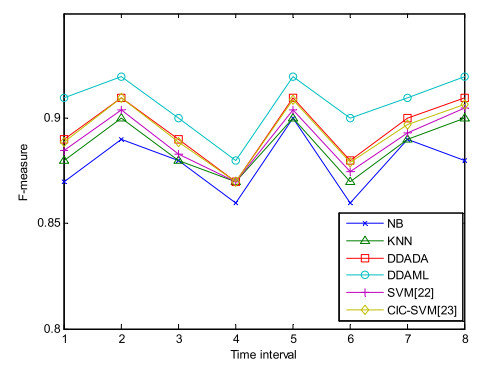
\includegraphics[scale=0.4]{fig28.png}\\
    \caption{Comparison of F-measure in different time intervals.}
    \label{fig:time}
\end{figure}

\subsubsection{2. ROC and AUC Curves}
A Receiver Operating Characteristic curve (ROC curve) shows the performance of a binary classifier system as its discrimination thresholds change in statistics. Plotting the True Positive Rate (TPR) against the False Positive Rate (FPR) at different thresholds creates the curve. AUC measures accuracy. This area's level is defined as follows.

\begin{figure}[H]
    \centering
    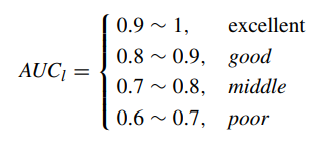
\includegraphics[scale=0.5]{fig29.png}
\end{figure}

Figure~\ref{fig:rccur} shows that FPR and TPR settings affect ROC curves for different algorithms. The NB and KNN algorithms cover a small area of the ROC curve for FPR and TPR settings, while the DDAML algorithm outperforms all other algorithms. 

\begin{figure}[H]
    \centering
    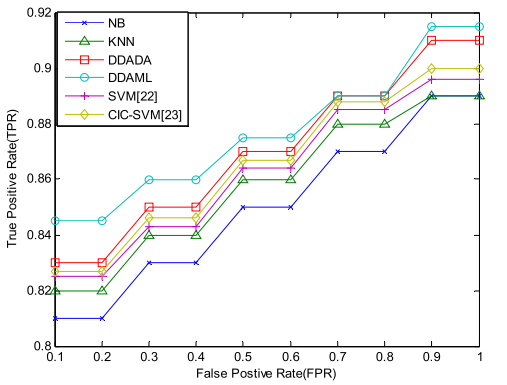
\includegraphics[scale=0.4]{fig30.png}\\
    \caption{Comparison of ROC curves.}
    \label{fig:rccur}
\end{figure}

Table~\ref{tab:croc} shows AUC values. DDAML's 0.912 AUC indicates excellent prediction. The NB, SVM, CIC-SVM, and DDADA algorithms also predict well with AUC values of 0.891, 0.893, 0.895, and 0.899. From the simulation experiments above, DDADA and DDAML algorithms in this paper outperform other DDoS attack detection algorithms.

\begin{table}[H]
    \centering
    \begin{tabular}{l r}
    \toprule
    Method & AUC \\
    \midrule
    NB & 0.981 \\
    KNN & 0.852  \\
    SVM & 0.983 \\
    CIC-SVM & 0.985 \\
    DDADA & 0.899 \\
    DDAML & 0.912 \\
    \bottomrule
    \end{tabular}
    \caption{Comparison of ROC curves.}
    \label{tab:croc}
\end{table}

\section{ADVANTAGES AND LIMITATIONS}

DDADA and DDAML DDoS detection algorithms have several advantages. The first advantage is accuracy. By measuring the degree of the attack and machine learning, the algorithms can accurately identify DDoS attacks. Table~\ref{tab:eva} shows that the True Positive Rate (TPR) values for DDADA and DDAML algorithms are 0.987 and 0.994, respectively, greater than those of the other algorithms (NB, KNN, SVM, CIC SVM). DDADA and DDAML algorithms have reduced False Positive Rate (FPR) values of 0.016 and 0.009, respectively. These DDADA and DDAML algorithms can help to improve the overall detection system. Speed is the next potential advantage. Figure~\ref{fig:time} shows that by evaluating the DDADA and DDAML approaches, DDoS attacks can be detected faster, reducing the network’s damage.\\

However, there are also some limitations to this approach. The first limitation is complexity. DDoS detection based on attack complexity takes a lot of computing capacity and processing power. This makes implementing a detection system harder and more expensive, especially for large organizations with significant traffic volumes. Machine learning algorithms require a lot of data to train, making them challenging to design and maintain for organizations without specialized skills. Another limitation is overhead.DDoS detection using a degree of attack complexity measure may increase network cost, affecting performance. Data processing and analysis to classify assaults by complexity can increase overhead. Training and updating a machine learning algorithm may require additional hardware or software, which might increase the cost of deploying and maintaining the detection system.\\


\section{IDENTIFICATION AND EXPLANATION OF RESEARCH GAPS}
Several research gaps can be addressed in the SDN field of DDOS attack detection. Here are some examples:

\begin{itemize}
    \item Improved detection methods:
    While there are several existing methods for detecting DDOS attacks in SDN, such as DDADA and DDAML, there is still room for improvement. For example, the research could focus on developing more accurate and adaptable algorithms that detect a more comprehensive range of DDOS attack types and behaviours.

    \item Real-time detection:
    One of the challenges in DDOS attack detection is detecting the attack as it is happening rather than after the fact. Research could focus on applying DDADA and DDAML algorithms for detecting DDOS attacks in real-time, which could enable faster response and mitigation.

    \item Scalability: 
    As networks grow and become more complicated, DDOS detection and mitigation systems must scale and adapt. Research could produce systems that can handle massive traffic and data quantities with great accuracy and performance.
    
\end{itemize}

\section{SUGGESTIONS FOR FUTURE ENHANCEMENTS}
There are several areas where enhancements could be made to improve the detection of DDOS attacks in SDN. Here are some examples:


\begin{itemize}
    \item To develop new detection methods, it is also helpful to explore ways to integrate existing methods or combine them in novel ways to create more robust and effective DDOS detection systems. By exploring a range of approaches, it may be possible to significantly improve the accuracy and effectiveness of DDOS detection in SDN.

    \item To develop algorithms that can analyze network traffic in real-time, using techniques such as packet inspection or flow analysis to identify patterns or anomalies that could indicate an attack. This could  allow the system to detect attacks as they happen, rather than after the fact.

    \item The potential enhancements that could improve scalability include optimizing algorithms and data structures for efficient processing, implementing efficient data storage and retrieval methods, and using techniques such as caching or pre-processing to reduce the amount of data that needs to be processed in real-time.
    
\end{itemize}


\section{CONCLUSION}
The defence against the DDoS attack depends on the ability to identify the attack. Recent DDoS attack detection technologies are inaccurate and susceptible to other causes. The authors’ accomplishments address the above issues: First, the authors suggested analyzing flow length, duration, size, and ratio when DDoS attack the SDN controller. The degree of attack is introduced for DDoS detection. The DDADA algorithm detects this concept. To improve DDoS attack detection, the DDAML algorithm is introduced. The authors' proposed algorithms detect DDoS attacks better than existing solutions. Finally, experimental results show that the DDAML algorithm outperforms the others on various performance measures.






 \bibliographystyle{apacite}
\bibliography{ref}{}
\end{document}

